\documentclass[12pt]{article}
\usepackage{amsmath, amssymb, geometry, tikz}
\usetikzlibrary{calc}
\geometry{a4paper, margin=1in}

% Title Information
\title{Kinematics of Satellite Collisions: Elastic Case}
\author{Daniel T. \& Achates (ChatGPT)}
\date{\today}

\begin{document}

\maketitle

\begin{abstract}
This report explores the kinematics of satellite collisions, focusing on the elastic collision scenario. Conservation of momentum and kinetic energy is analyzed, laying the groundwork for understanding collision dynamics in orbital mechanics. Future work will include modeling the collision trace on the Earth's surface.
\end{abstract}

\section{Introduction}
Satellite collisions, while rare, have significant implications for space operations, including debris generation and long-term orbital sustainability. Understanding the kinematics of these events is essential for risk assessment and mitigation strategies. This report begins with an analysis of elastic collisions, assuming conservation of both momentum and kinetic energy.

\section{Elastic Collisions in Orbital Mechanics}
An elastic collision is characterized by the conservation of both linear momentum and kinetic energy. In the context of satellite collisions, this assumption is valid for idealized cases where energy loss due to deformation or heat is negligible.

\section{Mathematical Formulation}

\subsection{Conservation of Momentum}
The law of conservation of linear momentum states:
\begin{equation}
    m_1 \vec{v}_{1i} + m_2 \vec{v}_{2i} = m_1 \vec{v}_{1f} + m_2 \vec{v}_{2f},
\end{equation}
where:
\begin{itemize}
    \item $m_1, m_2$: masses of the two satellites,
    \item $\vec{v}_{1i}, \vec{v}_{2i}$: initial velocities of the satellites,
    \item $\vec{v}_{1f}, \vec{v}_{2f}$: final velocities of the satellites.
\end{itemize}

\subsection{Conservation of Kinetic Energy}
For elastic collisions, the total kinetic energy before and after the collision remains constant:
\begin{equation}
    \frac{1}{2} m_1 |\vec{v}_{1i}|^2 + \frac{1}{2} m_2 |\vec{v}_{2i}|^2 = \frac{1}{2} m_1 |\vec{v}_{1f}|^2 + \frac{1}{2} m_2 |\vec{v}_{2f}|^2.
\end{equation}

\section{Derivation of Final Velocities}
Using the principles of momentum and energy conservation, the final velocities can be expressed as:
\begin{align}
    \vec{v}_{1f} &= \frac{(m_1 - m_2) \vec{v}_{1i} + 2 m_2 \vec{v}_{2i}}{m_1 + m_2}, \\
    \vec{v}_{2f} &= \frac{(m_2 - m_1) \vec{v}_{2i} + 2 m_1 \vec{v}_{1i}}{m_1 + m_2}.
\end{align}

\section{Frames of Reference}

\subsection{Inertial Frame vs. Center of Mass Frame}

\paragraph{Inertial Frame.} In the inertial frame, the velocities $\vec{v}_{1}$ and $\vec{v}_{2}$ are defined relative to a fixed observer. While intuitive, solving elastic collisions in this frame can become algebraically intensive.

\paragraph{Center of Mass Frame.} The center of mass (CoM) frame simplifies calculations by transforming the velocities such that:
\begin{equation}
    \vec{v}_{\text{CoM}} = \frac{m_1 \vec{v}_{1i} + m_2 \vec{v}_{2i}}{m_1 + m_2}.
\end{equation}
In this frame:
\begin{itemize}
    \item The total momentum of the system is zero: $\vec{P} = 0$.
    \item Velocities before and after the collision are symmetric about the CoM.
\end{itemize}

\paragraph{Transformations.} Transforming to the CoM frame:
\begin{equation}
    \vec{v}_{i, \text{CoM}} = \vec{v}_{i} - \vec{v}_{\text{CoM}}.
\end{equation}
Transforming back to the inertial frame after solving:
\begin{equation}
    \vec{v}_{i}^{\prime} = \vec{v}_{i, \text{CoM}} + \vec{v}_{\text{CoM}}.
\end{equation}

\section{Collision Energy vs. Crossing Angle}
The collision angle $\theta$ (the angle between the initial velocity vectors) determines the relative velocity and energy distribution. Using the law of cosines:
\begin{equation}
    |\vec{v}_{\text{rel}}|^2 = |\vec{v}_{1}|^2 + |\vec{v}_{2}|^2 - 2|\vec{v}_{1}||\vec{v}_{2}|\cos\theta.
\end{equation}
Special cases:
\begin{itemize}
    \item $\theta = 0^\circ$: Head-on collision.
    \item $\theta = 90^\circ$: Orthogonal trajectories.
    \item $\theta = 180^\circ$: Opposite directions (maximum relative velocity).
\end{itemize}

\subsection{Graph: Collision Energy vs. Crossing Angle}
A plot of relative collision energy $|\vec{v}_{\text{rel}}|^2$ vs. crossing angle $\theta$ provides insights into the geometry of collisions. This visualization will be included in future work.

\section{Law of Cosines Diagram}
Below is a diagram illustrating the law of cosines for the relative velocity:

\begin{center}
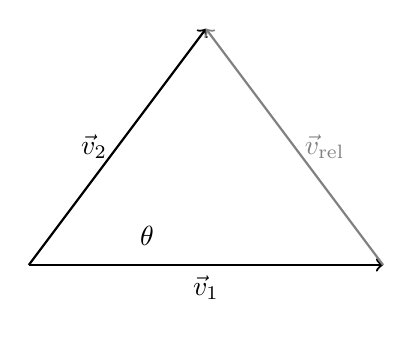
\begin{tikzpicture}[scale=1.5]
    \draw[thick, ->] (0, 0) -- (3, 0) node[midway, below]{$\vec{v}_1$};
    \draw[thick, ->] (0, 0) -- (1.5, 2) node[midway, left]{$\vec{v}_2$};
    \draw[thick, ->, gray] (3, 0) -- (1.5, 2) node[midway, right]{$\vec{v}_{\text{rel}}$};
    \node at (1, 0.25) {$\theta$};
\end{tikzpicture}
\end{center}

\section{Applications to Satellite Collisions}
Elastic collision analysis is a useful starting point for understanding post-collision trajectories of satellites. While real-world collisions often involve some inelasticity, the elastic model provides insights into the dynamics of high-energy interactions.

\section{Future Work}
Future studies will:
\begin{itemize}
    \item Extend the analysis to inelastic collisions, accounting for energy dissipation.
    \item Integrate numerical simulations and Mathematica-generated diagrams.
    \item Model the collision trace on the Earth's surface.
\end{itemize}

\end{document}
